\part{Vers une synergie homme-machine}
    
À l'heure actuelle l'IA est assez avancée pour qu'elle puisse gérer
des tâches répétitives avec une quantité de données de référence importante
en utilisant son réseau neuronal lui permettant d'interpréter une démarche, un comportement à suivre. \newline

Il faut que les données d'entrée et de sortie soient bien définies pour aboutir
à une réponse logique et cohérente, à un cas particulier donné,
et qui soit basée sur des statistiques et des probabilités. \newline

Ainsi, une base de données de multiples mammographies avec leurs diagnostiques
associés permettra de lire les nouveaux clichés avec établissement d'un risque cancéreux. \newline

Le développement de l'Intelligence Artificielle aura des conséquences sur le Marché du Travail avec des emplois en déclin,
avec d'autres emplois concernés mais sans disparition de postes, mais aussi avec une croissance pour le recrutement de certains postes.
Ces modifications auront des répercussions socio-économiques, politiques et légales. \newline

\chapter{Les conséquences sur l'Emploi}
    \section{Les emplois concernés par le remplacement par l'Intelligence Artificielle}

    L'IA s'applique plus facilement aux emplois à faible valeur ajoutées,
    présentant des tâches répétitives avec peu de réflexion et ne prenant pas en compte des paramètres externes ou variables. \newline

    Cet avis est partagé par le docteur Tom Mitchell de l'université Carnegie Melon dans un article sur l'impact
    du Machine Learning sur les différentes professions \newline

    Une Intelligence Artificielle prendra mieux en charge un poste de chauffeur taxi ou de chauffeur routier
    étant donné l'absence de fatigabilité par rapport à l'humain qui doit règlementairement prendre des pauses régulières
    pendant la conduite, pénalisant ainsi la durée du transport et par conséquence sa rentabilité. \newline

    Amazon a créé récemment des commerces de proximité où le client entre en s'identifiant grâce à une application sur son smartphone,
    et où il se sert directement dans les rayons. Les caméras reconnaissent le client et les articles qu'il récupère dans son panier,
    ou qu'il repose. En ressortant, l'acheteur paye en repassant son smartphone sur les mêmes portiques.
    Le magasin se passe ainsi de caissières, réduisant les coûts de charges salariales.
    \footnote{source: \url{https://money.cnn.com/2018/01/26/technology/amazon-go-store/index.html}}
    \newline

    \begin{figure}[H]
        \centering
        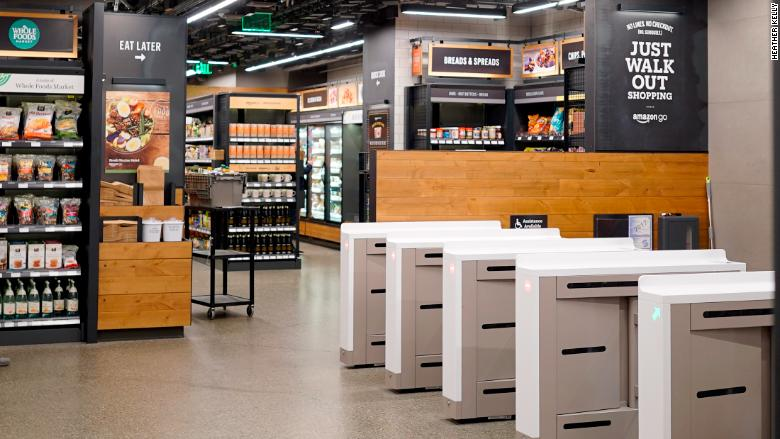
\includegraphics[width=0.7\textwidth]{Images/amazongoinside}
        \caption{Photographie montrant le système de portique d'achat d'un magasin Amazon Go}
        \label{fig:explicability}
    \end{figure}

    Jusqu'alors nous réfléchissions en perte d'emplois, mais il faut également penser en prise en charge
    et d'accompagnement dans la réalisation de tâches. \newline

    La disparition de certaines activités professionnelles nécessitera une reconversion vers d'autres emplois plus demandeurs
    (services à la personne, santé et bien-être). \newline

    Les pertes d'emplois sont inévitables, cependant les conditions de travail iront en s'améliorant.
    On pourra s'attendre à moins d'accidents professionnels, en raison d'une réduction de la pénibilité au travail. \newline

    \section{Les emplois modifiés par l'Intelligence Artificielle}

    Les emplois décisionnels ne seront pas impactés en termes de perte d'emplois. L'Intelligence Artificielle agira plus
    comme une aide décisionnelle fournissant des indicateurs clés qu'elle aura calculée, mais également des préconisations
    d'actions ou de choix à prendre. On peut parler d'Intelligence Augmentée lorsque l'Intelligence Humaine est aidée par
    l'Intelligence Artificielle. \newline

    Les professions demandant de nombreuses connaissances en rapport avec l'Humain seront également préservées.
    On retrouve dans cette liste, les professions juridiques (juges, avocats, notaires), médicales (médecins, psychologues, infirmières),
    ou encore du domaine des ressource humaines (formateur, coach, responsable RH). \newline

    Les métiers de l'artisanat, où la création nécessitant des gestes techniques non répétitifs et un esthétisme propre à chaque réalisation,
    comme les bijoutiers, verriers, menuisiers ou ferronniers ne sont pour le moment pas égalables par l'Intelligence Artificielle.
    En effet les métiers artistiques et créatifs ne sont occupables que par des humains, étant donné que seuls ces derniers
    possèdent une capacité créative et imaginative, même si des essais de créations (musicales et picturales notamment) ont été tentés par
    L'Intelligence Artificielle. \newline

    Dans l'industrie du luxe (par exemple la bijouterie, la haute-couture, la maroquinerie ou encore le prêt-à-porter) la notion de fabriquer à la main
    un produit pourrait devenir un argument de vente auprès des consommateurs, comme peut l'être le "Made in France" de nos jours. \newline

    La recherche d'emploi bénéficie également des compétences de l'Intelligence Artificielle. Cette dernière améliore le processus, en analysant
    les données qu'elle perçoit sur les CVs et en les accordants avec les critères de recherche fournies par l'émetteur de la demande (recruteurs
    ou chasseur de têtes). Cette technique est par ailleurs déjà utilisée dans certaines entreprises de recherche d'emploi et de recrutement
    (Indeed, LinkedIn). \newline

    \newpage

    \section{Les emplois créés par l'essor de l'Intelligence Artificielle}

    Une des conséquences directes du développement de l'Intelligence Artificielle est la création de nouveaux postes.
    En effet en réponse à la demande croissante de l'Intelligence Artificielle, il est nécessaire de mettre en place
    de nouvelles infrastructures physiques. Ces dernières doivent être maintenues et mises à jour régulièrement par des techniciens.
    De plus pour concevoir et mettre en place la logique de ces infrastructures, le fonctionnement, le code, il est également nécessaire de
    faire appel à des architectes, des data scientists et des développeurs. Enfin ces développeurs se doivent de posséder des connaissances
    en sécurisation. Des experts en sécurité pourront au choix être recrutés ou mandatés au près de prestataires externes. \newline

    En septembre 2018 le World Economic Forum, une fondation a but non-lucratif organisant tous les ans le Forum de Davos,
    et siègeant à Genève, a publié dans un article que d'ici 2022 75 millions d'emplois seraient détruits à l'échelle mondiale et
    que 133 millions autres emplois seraient créés, soit une croissance de 58 millions d'emplois.
    \footnote{source: \url{https://www.oezratty.net/wordpress/2018/fumeuses-previsions-futur-emploi-et-ia/}}
    \newline

    \begin{figure}[H]
        \centering
        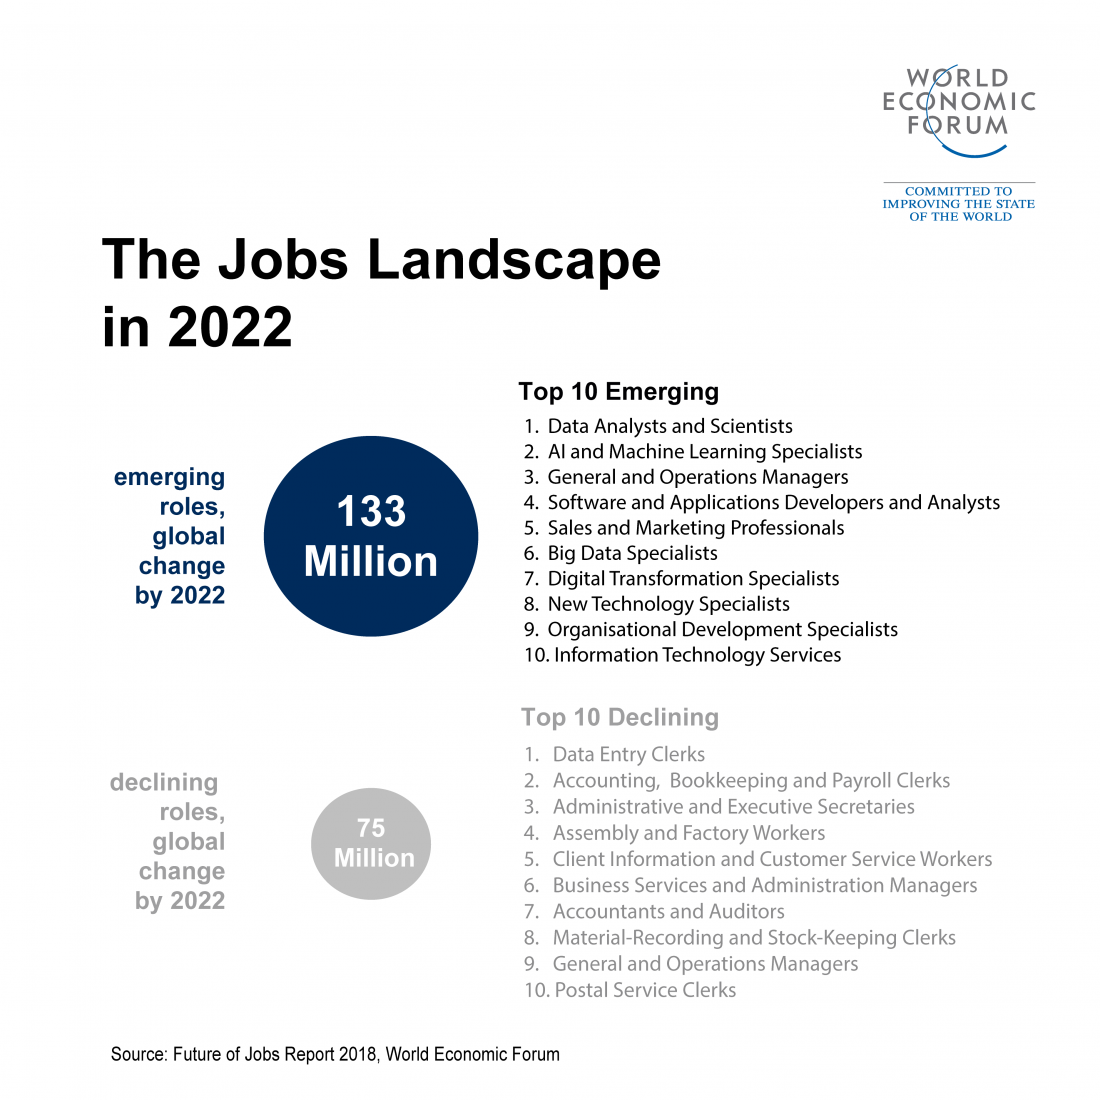
\includegraphics[width=0.7\textwidth]{Images/futurejobs}
        \caption{Résultat de l'étude du WEF avec répartition des emplois impactés et créés}
        \label{fig:explicability}
    \end{figure}

\chapter{Les conséquences socio-économiques et légales}

    Historiquement l'automatisation des années 1900 ont engendré de nombreuses luttes sociales, grèves, front populaire.
    Si le changement lié à l'Intelligence Artificielle est massif et rapide, il se peut que les mêmes conséquences se reproduisent.
    Plusieurs économistes tablent sur ce changement rapide du paysage dans les 10 années à venir. \newline

    En Mai 2016, l'OCDE publie une étude qui prévoit que 9\% des emplois français à ce moment-là sont complètement automatisables.
    Ce qui peut être mis en balance avec le taux de chômage actuel en France qui avoisine les 9\%.
    L'étude montre aussi que l'approche par métiers ou par tâches ne débouche pas sur les mêmes résultats. Le taux de la population impacté,
    en fonction du taux de possibilité d'automatisation n'est pas le même dans les deux cas.
    \footnote{source: \url{https://www.oecd-ilibrary.org/docserver/5jlz9h56dvq7-en.pdf?expires=1549828830&id=id&accname=guest&checksum=36F9D06A8C9917FA4D2D2D7E2DBB2F01}}
    \newline

    \begin{figure}[H]
        \centering
        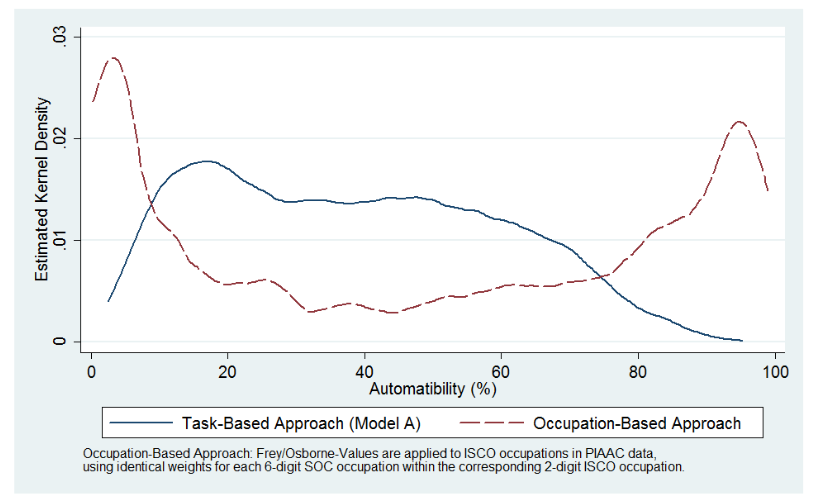
\includegraphics[width=0.7\textwidth]{Images/approcheparpostevsapprochepartache}
        \caption{Représentation des résultats de l'étude de McKinsey}
        \label{fig:explicability}
    \end{figure}

    En décembre 2017 McKinsey évalue la perte d'emploi en raison de l'automatisation par l'Intelligence Artificielle à 7 millions aux États-Unis
    en 3 ans. Cela donne une idée de l'évolution de la répartition des différents secteurs de travail entre 2016 et 2020.
    \footnote{source: \url{https://www.oezratty.net/wordpress/2018/fumeuses-previsions-futur-emploi-et-ia/}} \newline

    \begin{figure}[H]
        \centering
        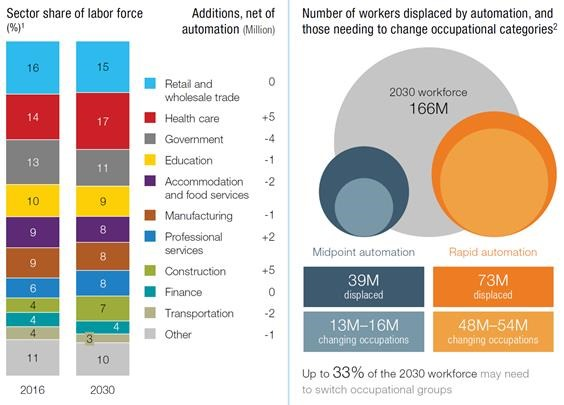
\includegraphics[width=0.7\textwidth]{Images/laborforceevolution}
        \caption{Représentation des résultats de l'étude de McKinsey}
        \label{fig:explicability}
    \end{figure}

    En octobre 2018, le Gartner Group prévoit que le solde entre création et destruction d'emploi lié à l'Intelligence Artificielle
    commencera à être positif à partir de 2020.
    \footnote{source: \url{https://www.oezratty.net/wordpress/2018/fumeuses-previsions-futur-emploi-et-ia/}} \newline

    \begin{figure}[H]
        \centering
        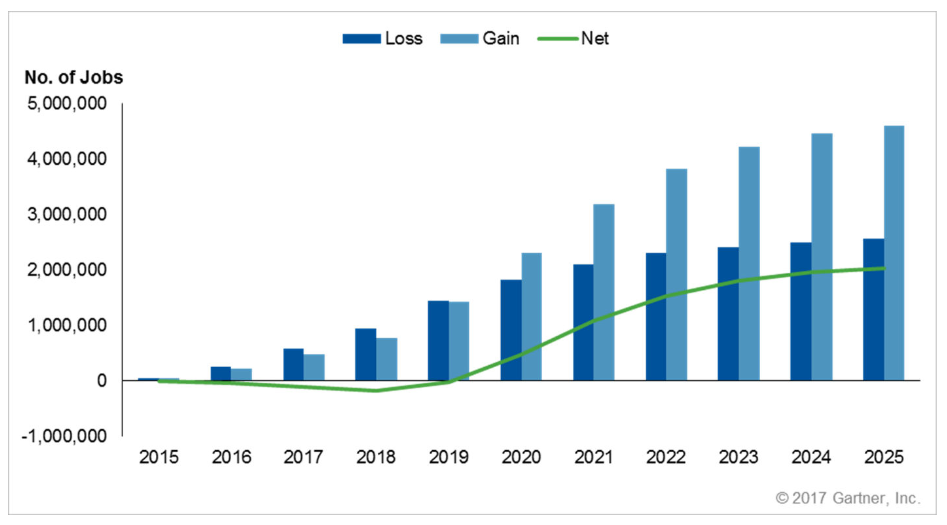
\includegraphics[width=0.7\textwidth]{Images/gartneraiandfuturework}
        \caption{Graphique des résultats de l'étude du Gartner Group en 2018}
        \label{fig:explicability}
    \end{figure}

    Politiquement l'État en collaboration avec l'Éducation Nationale et l'Éducation Supérieure devra prendre en compte l'essor de l'Intelligence
    Artificielle au niveau du lycée et des études supérieures afin d'améliorer le socle de base de connaissances en informatique et
    d'orienter vers les emplois à plus grande valeur ajoutée. L'État devra également favoriser le maintien des spécialistes en France. \newline

    Sur le plan législatif certains textes devront être modifiés afin de prendre en compte l'Intelligence Artificielle,
    Actuellement, il existe zone grise lors d'accidents impliquants les véhicules autonomes. La responsabilité incombe-t-elle au propriétaire
    du véhicule ou à son fabriquant ? \newline

    Les différentes simulations économiques à moyen terme précédemment citées posent différents problèmes :

    \begin{itemize}
        \item Beaucoup de ces projections sont liées à des sondages interrogeant principalement des cadres-responsables, et sont plus des
        enquêtes d'option que de vrai enquêtes scientifiques.\newline
        \item L'étude Oxford 2013 a été critiquée car elle parle de métiers sans les décomposer en tâches. À mi-parcours, nous sommes bien
        loin des prédictions années pour 2023.\newline
        \item Presque aucune étude n'a pris en compte la possibilité d'évènements ayant une influence majeure l'économie mondiale (comme par exemple
        le Brexit). \newline
    \end{itemize}

    Le développement de l'Intelligence Artificielle intéresse également les différentes forces armées dans le monde. Avec des robots militarisés,
    en théorie pour diminuer le nombre de morts sur le champs de bataille, mais qui ne tueront pas que d'autres robots, ce qui rentre en contradiction
    avec les trois lois de la robotique énoncées par Isaac Asimov. \newline